% !TEX TS-program = pdflatex
% !TEX root = ../Tesis.tex
%*****************************************
\chapter{State of the Art}\label{ch:stateofart}
%*****************************************
We have already stated the motivation and objectives of this thesis. Now, we will describe in detail some of the more relevant issues for the state of the art. First, in section~\ref{sec:neuroimaging}, we will make an introduction to the different neuroimaging modalities used in our experiments. Afterwards, we will provide some insights into the neurological and psychiatric disorders treated here in section~\ref{sec:disorders} or the most extended voxel-wise analyses used in the neuroimaging community at section~\ref{sec:vwanalyses}. Finally, at section~\ref{sec:machinelearning} we will explore recent contributions to the field that use Machine Learning. 

\section{Introduction to Neuroimaging}\label{sec:neuroimaging}
Medical imaging refers to all types of 2D, 3D and 4D images used in clinical practice. These involve many different modalities, among them X-rays, ultrasound, endoscopy, microscopy, etc. In neuroimaging, the most extended is by far \ac{MRI}, which provides intensity maps that represent the internal structure of the brain. Other modalities are aimed at studying the function of the brain, by injecting radioactive ligands that, bound to a receptor, can measure its distribution. This is the case of \ac{PET} and \ac{SPECT}.

\subsection{\acf{MRI}}
\acf{MRI} is perhaps the most widespread modality in neuroimaging, given its ability to visualize both structural and functional (in functional \ac{MRI}) properties of the brain, and, in contrast to other imaging modalities that use radiotracers, is considered non-invasive. \ac{MRI} uses strong magnetic fields to excite certain atomic nuclei, that can absorb and emit this energy. 

\begin{figure}[htp]
	\centering
	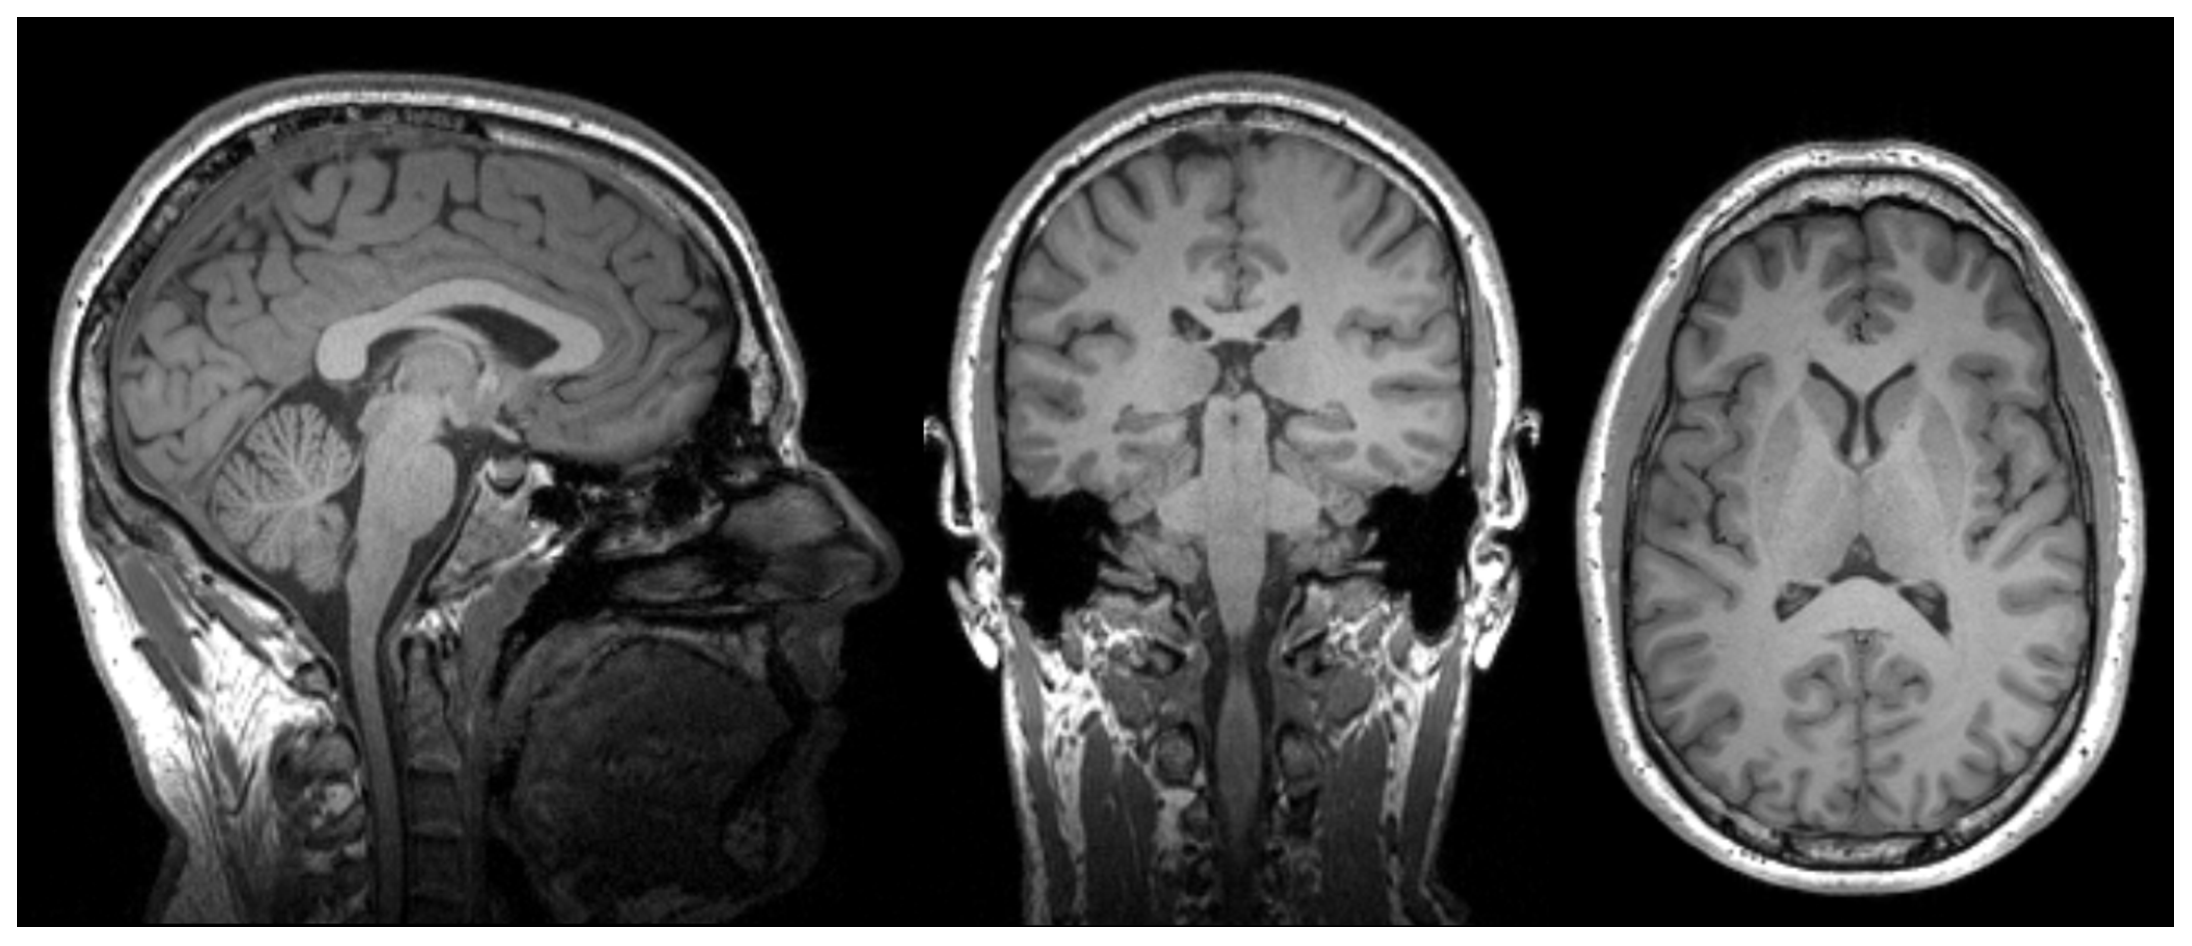
\includegraphics[width=0.7\linewidth]{Graphics/ch2/example_MRIT1}\\
	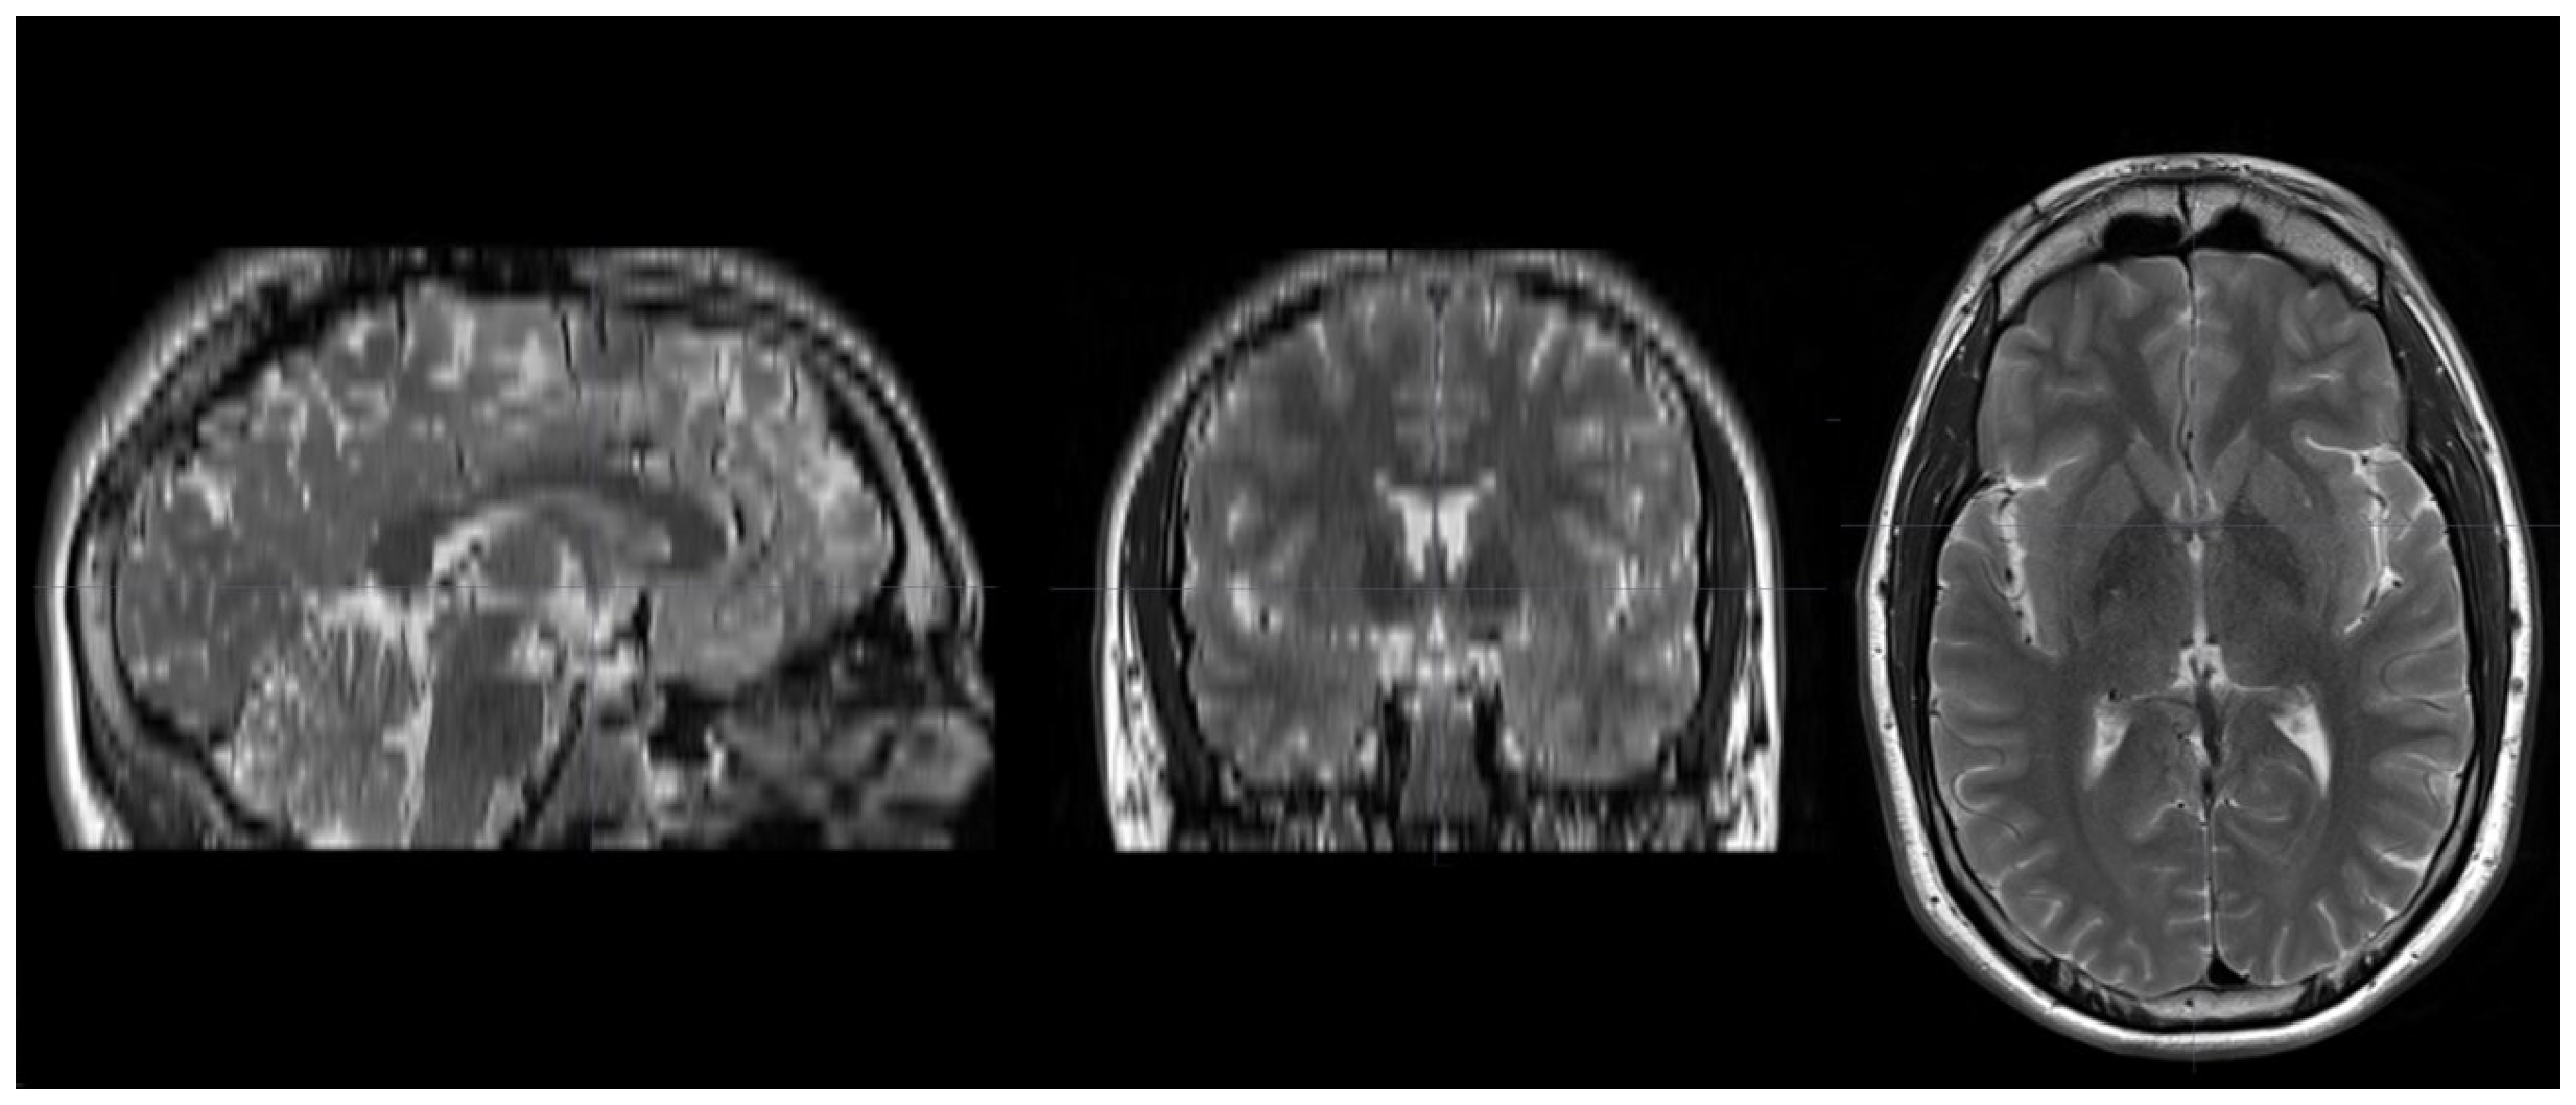
\includegraphics[width=0.7\linewidth]{Graphics/ch2/example_MRIT2}
	\caption[Example of T1 and T2-weighted \acs{MRI} images.]{Example of T1 and T2-weighted \ac{MRI} images of the same subject (me).}
	\label{fig:example_MRI}
\end{figure}

\ac{MRI} combines a constant magnetic field with a \ac{RF} emission to excite the atomic nuclei present in corporal structure, resulting in a image of the distribution of certain atoms in the body. Most \ac{MRI} systems use hydrogen atoms, since they are present in water (which adds up to around 70\% of body mass) and the signal derived is stronger than other atoms, increasing the \ac{SNR}, and therefore, the image quality. 

The procedure uses a strong magnetic field $B_0$ to align the magnetic moment of the hydrogen nuclei in parallel or anti-parallel (depending of their initial spin). This way, the magnetic moment of all nuclei will increase up to a stable state, in contrast to their null value in absence of $B_0$. Within this magnetic field, the hydrogen atoms precess around an axis along the direction of the field. 

A given nuclei has a resonance frequency which is proportional to the intensity of $B_0$, which, by using strong fields, allow us to resonate hydrogen far below potentially damaging frequencies. The precession frequency is determined by the Larmor equation (\ref{eq:lamor}):

\begin{equation}\label{eq:lamor}
f_0 = \frac{\gamma}{2\pi } B_0 
\end{equation}
where $\gamma$ depends on the nuclei, which in the case of hydrogen, $\gamma = 42.6$ MHz/T. When a subject is introduced in the \ac{MRI} scanner, it is submitted to the magnetic field $B_0$, so that the hydrogen nuclei are aligned to the field, with a precession frequency $f_0$. Then, a \ac{RF} pulse of the same frequency is generated, which is then absorbed by the nuclei, forcing them to place perpendicular to the field. Once the \ac{RF} emission is interrupted, the nuclei return to its equilibrium state by means of a procedure called relaxation. In this procedure, they emit part of the absorbed energy, which is then captured by a \ac{RF} receptor. Usually, position information is encoded in the \ac{RF} signal by varying $B_0$ using gradient coils. 

The \ac{RF} signal is measured during the relaxation time, and two different relaxation times are set: the T1 (spin-lattice) relaxation time and the T2 (spin-spin) relaxation time. The T1 time is the time during which nuclei emit energy to the adjacent tissue and realign to the longitudinal plane (z axis), whereas the T2 time refers to the time when nuclei realign to the transversal plane (y axis). These times are used to create T1-weighted and T2-weighted images (see Figure~\ref{fig:example_MRI}). T1-weighted images allow to distinguish between \ac{GM} and \ac{WM} in the cerebral cortex, to identify fatty tissue, and generally, obtain structural information. Conversely, T2-weighed images are used to assess \ac{CSF} or to visualize and identify \ac{WM} lessions. 

\subsection{\acf{SPECT}}
The \acf{SPECT} is based on the principles of \ac{CT}, by which a series of signal acquisitions at different angles can be reconstructed back into a bidimensional distribution of the signal. In \ac{SPECT}, a gamma photon emitting radioisotope is linked to a pharmaceutical that binds to a given biomarker, generating a radiopharmaecutical or agent. This agent is injected into the patient, and after a certain time in which the radiopharmaceutical is distributed, the patient is introduced into the \ac{SPECT}-\ac{CT} scan. 

Afterwards, the scanner performs a series of acquisitions at different planes and angles from the body, from which the gamma signal is measured. For each plane, all acquisitions at each angle are pooled and a single two-dimensional image is reconstructed using a \ac{FBP} algorithm, or Radon inversion formula \cite{Herman2009l}, which derives from the Fourier's Theorem. A total of 180 projections per plane, using an angular resolution of 2 degrees, are usually taken. 

There exist a wide variety of radiopharmaceuticals used in clinical practice, and therefore, we will only focus on the two varieties used in this thesis. First, we use an agent called $^{99m}$Tc-HMPAO, which consists of two stereoisomers of hexametazime (HMPAO) linked to the radioisotope technetium 99-metastable. This agent is usually used to assess \ac{rCBF}, which can be used to diagnose neurological diseases or cancer. 

\begin{figure}[p]
	\centering
	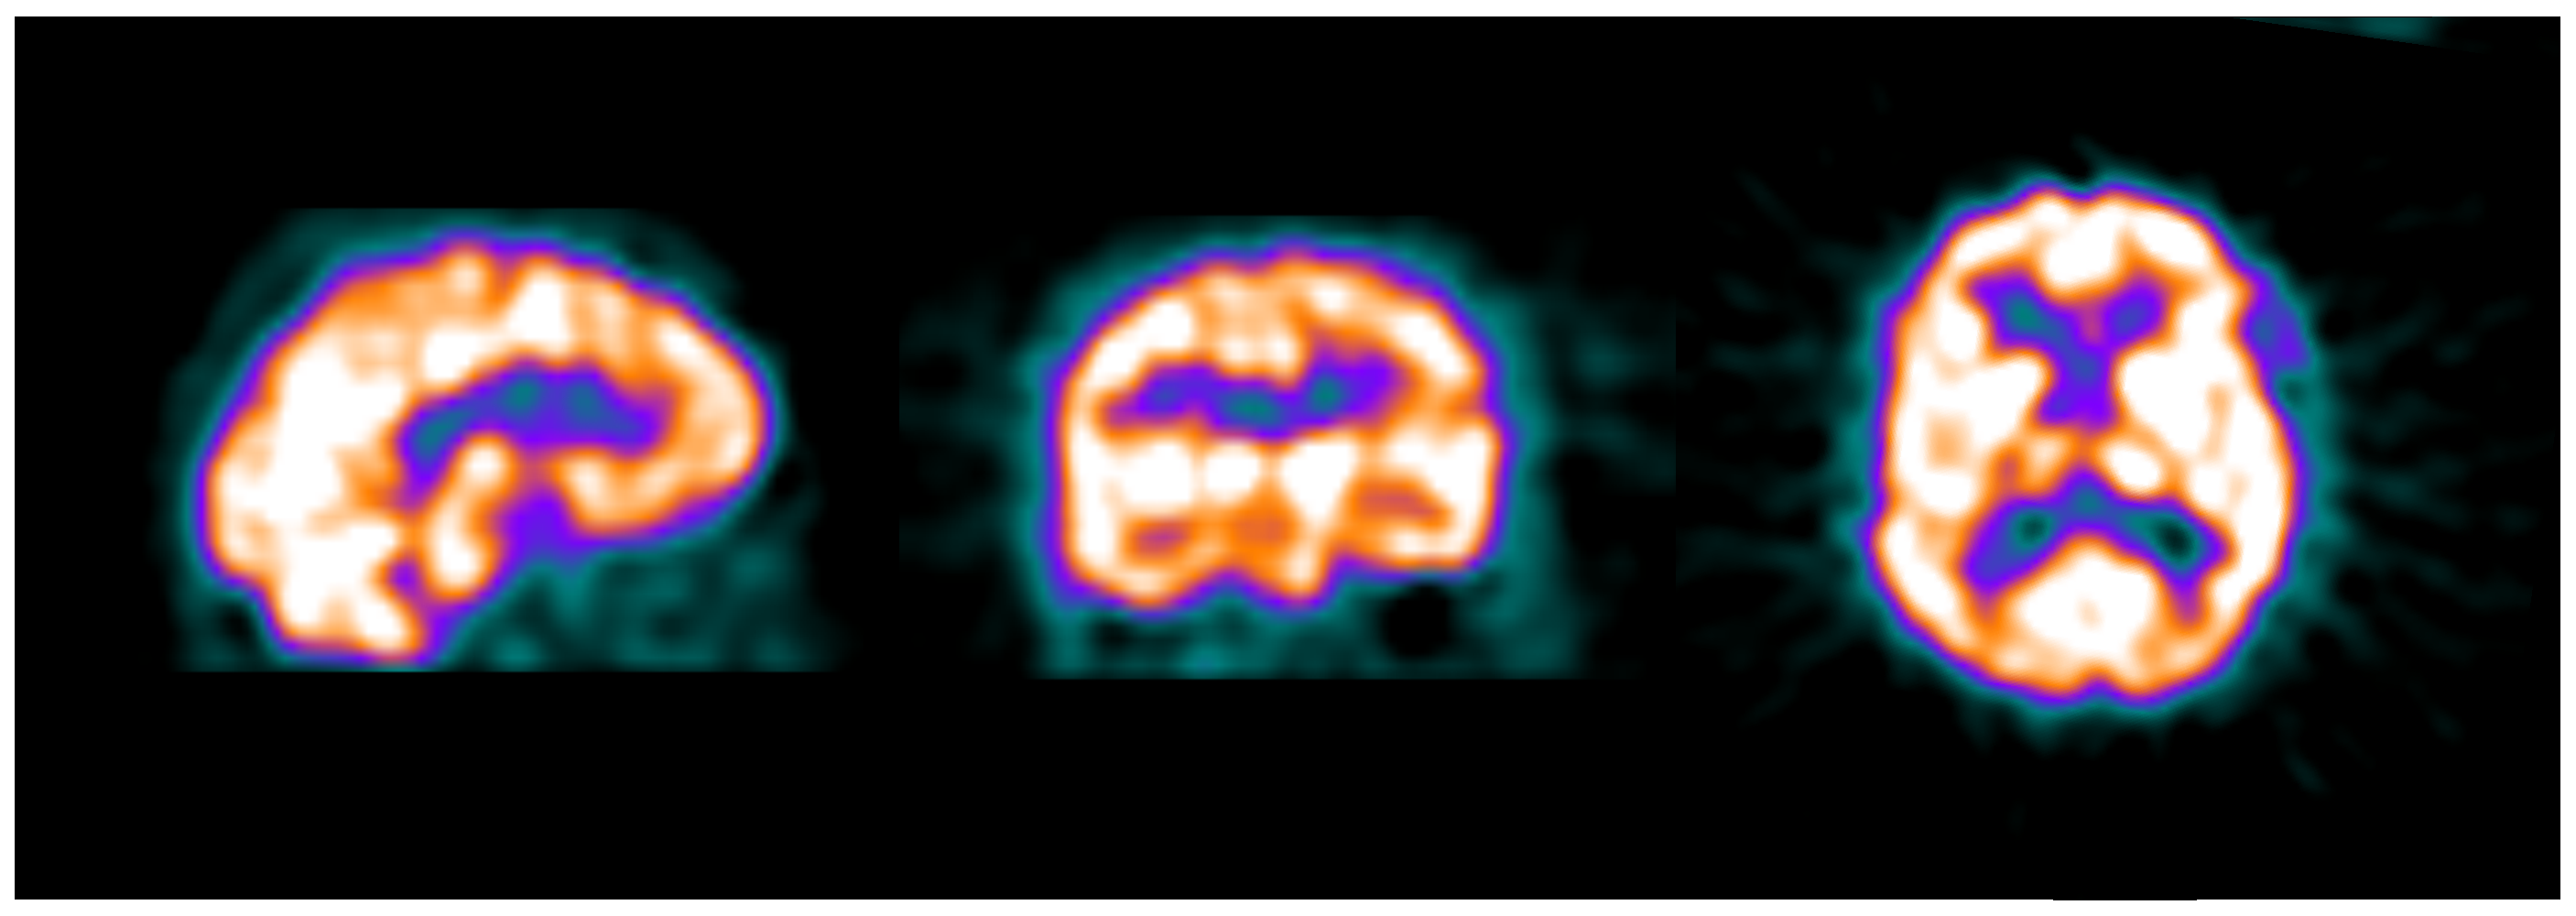
\includegraphics[width=0.8\linewidth]{Graphics/ch2/example_SPECT}\\
	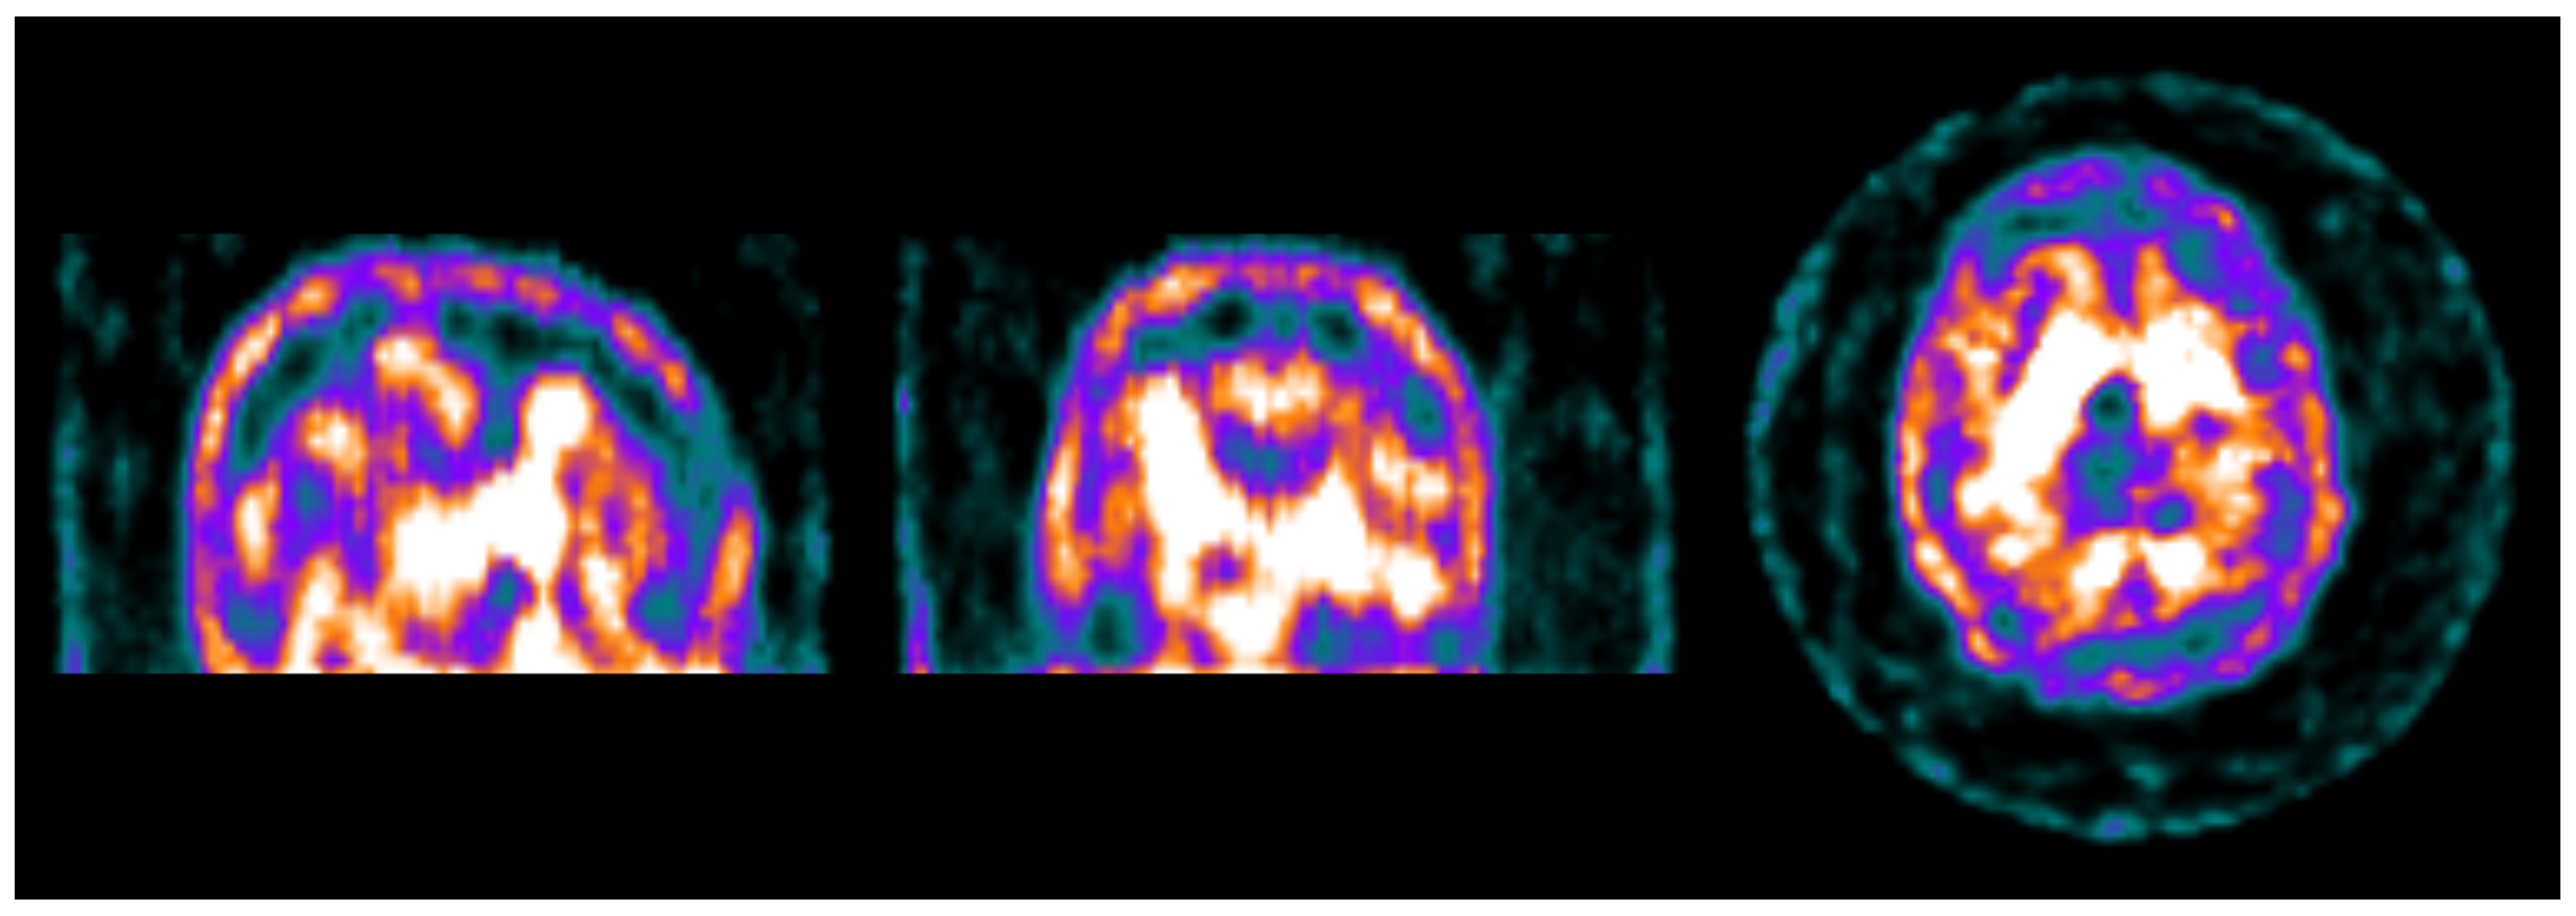
\includegraphics[width=0.8\linewidth]{Graphics/ch2/example_DaTSCAN}
	\caption[Example of \acs{SPECT} images.]{Example of \acs{SPECT} images, a \acs{SPECT}-HMPAO and a \acs{SPECT}-DaTSCAN.}
	\label{fig:example_SPECT}
\end{figure}

Additionally, we use images generated using the agent Ioflupane ($^{123}$I), a cocaine analog with high binding affinity for \ac{DAT}. It is commonly known for its tradename, DaTSCAN, and is used fundamentally in the assessment of \ac{PD}, given that the disease is associated with a loss of dopaminergic neurons in the striatal region. 

\subsection{\acf{PET}}
The \acf{PET} is a technique similar to \ac{SPECT}, but in this case, the agent used and the equipment is designed to deal with a pair of gamma photons resulting of the annihilation of a positron with its corresponding antiparticle, the electron. The pair of photons are generated in opposite directions, and the detection depends on them being simultaneously or coincidently detected at the receptor. The receptor comprises a scintillator which emits light when the gamma photon incides, and a detector, usually a photomultiplier tube or silicon avalanche photodiodes.

It uses the same \ac{FBP} algorithm as \ac{SPECT} in the reconstruction of the images, and a similar strategy for acquiring the signal at different angles. However, the amount of data is smaller than in \ac{SPECT}, and therefore, the reconstruction procedure is harder. As a result, \ac{PET} scanner operation is considered more costly than \ac{SPECT} \cite{Carlson2016}.  

\begin{figure}[p]
	\centering
	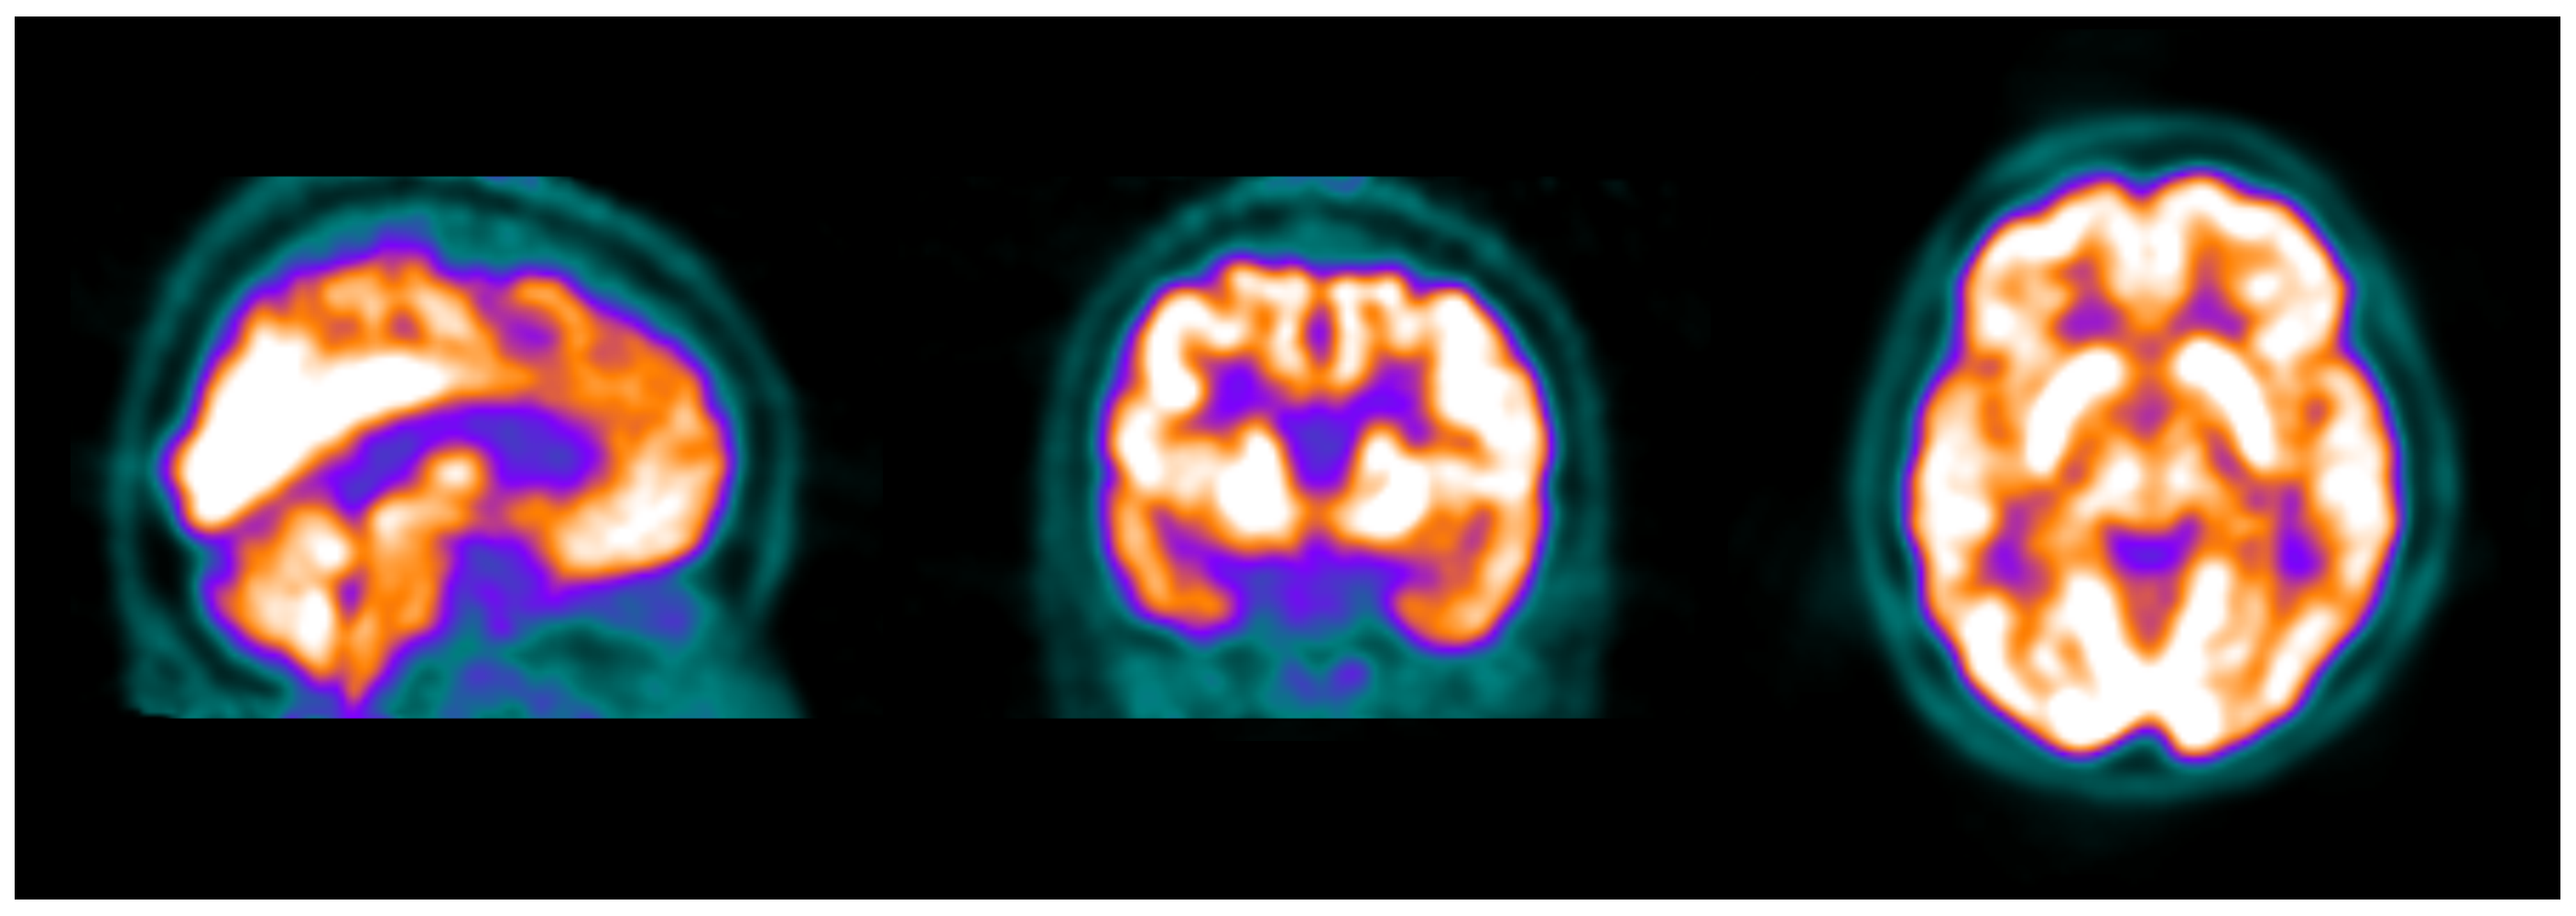
\includegraphics[width=0.8\linewidth]{Graphics/ch2/example_PET}
	\caption[Example of a \acs{PET}-FDG image.]{Example of a \acs{PET}-FDG image.}
	\label{fig:example_PET}
\end{figure}

The agent used in the images that we have processed is Fludeoxyglucose ($^{18}$F or FDG). It is a glucose analogue that allows us to measure the glucose metabolism in the brain. It is widely used in neurology \cite{Newberg2002} and cancer detection \cite{Kelloff2005}, since it can be correlated with cellular activity. 

\origsection{Medical Background}\label{sec:disorders}
\subsection{\acf{AD}}
\acf{AD} is the most common cause of dementia in the world, with more than 46 million people affected, and it is likely to increase up to 135.5 million by 2050 \cite{Association2016}. Its causes are still not clear, but it is characterized by deposits of high amounts of structures such as Amyloid-$\beta$ (A$\beta$) plaques or neurofibrillary tangles accompanied by synaptic dysfunction and neurodegeneration that eventually lead to cell death \cite{Ballard2011,Sevigny2016}.

Diagnosis of \ac{AD} is often based on the clinical history of the patient, using cognitive tests along with medical imaging and blood tests. A definite diagnosis can only be addressed post-mortem, via a direct examination of the brain tissue \cite{Ballard2011}. Cognitive tests such as \textit{Mini Mental State Exam} or \textit{Clinical Dementia Ratio} are widely used in clinical practice. 

Initial symptoms of \ac{AD} are often mistaken for normal ageing, in what is known as \acf{MCI}. Not all \ac{MCI}-affected subjects develop \ac{AD}. In fact, the prediction of \ac{MCI} conversion is the most urging challenge in \ac{AD} research, since an early diagnosis can lead to an improvement in life expectancy and quality of life of the patients. 

% Rewrite
\ac{MRI} brain images have been extensively used in the diagnosis of \ac{AD} by assessing neurodegeneration on \ac{GM} and \ac{WM} tissues. Research has shown in \cite{Baron2001,Misra2009,Pievani2013,Dubois2007} that neurodegeneration in Alzheimer's Disease mainly occurs in the \ac{GM} tissue. Particularly grey matter loss has been described in the hippocampus and parahippocampal gyrus, according to the NINCDS-ADRDA criteria for AD diagnosis \cite{Dubois2007}, with further atrophy described in the medial temporal structures, the posterior cingulate gyrus and adjacent precuneus \cite{Baron2001}. Moreover, significantly lower volumes of certain regions in \ac{GM} and \ac{WM} have been considered a promising biomarker and predictor of the progression of \ac{AD} in a longitudinal study involving \ac{MCI} patients \cite{Misra2009}, and some structures in the striatum (putamen and caudate nucleus) have shown important volume abnormalities \cite{Pievani2013}. All these data suggest that many of the symptoms of \ac{AD} can be observed in anatomical \ac{MRI} images even in early stages of the disease, which could be of great help in its successful diagnosis and treatment. 

Nuclear imaging, such as \ac{PET} or \ac{SPECT}, have also been used in clinical practice, especially to discard other diseases. In typical \ac{PET}-FDG or \ac{SPECT}-HMPAO, \ac{AD} is characterized by reduced brain activity in bilateral regions, such as the posterior cingulate gyri and precunei, as well as the temporo-parietal region \cite{Claus1994}. It also affects the frontal cortex and the whole brain in severe cases \cite{Leon1983,Kogure2000}. 

Recently, new more specific radiopharmaceuticals have been developed, among them the Pittsburgh compound B (PiB). This drug binds to fibrillar A$\beta$ allowing \textit{in vivo} visualization of A$\beta$ plaques in the brain \cite{Ikonomovic2008}. However, due to their technical requirements -a relatively small half-life of the radioactive element-, they are unusual in clinical practice. 

% DONE

\subsection{\acf{PKS}}
\acf{PKS} or Parkinsonian Syndrome is the second most common neurodegenerative disease in the world, with a prevalence of 1-3\% in the elder population (over 65 years)\cite{Eckert2007}. It is characterized by hypokinesia, rigidity, tremor and postural instability \cite{Eckert2007}. It is not a single disease itself, but a wide range of conditions that share similar symptoms. The most common cause of \ac{PKS} is \acf{PD}, but other possible causes include toxins, a few metabolic diseases, and other extrapyramidal syndromes such as Multiple System Atrophy, Progressive Supranuclear Palsy or Cortico-Basal Degeneration \cite{Christine2004,tatsch2008extrapyramidal}. 

\subsubsection{\acf{PD}}
The etiology of \acf{PD} involves the progressive loss of \acf{DAT} of the nigrostriatal pathway. This causes a decrease in the dopamine content of the striatum, since the pathway connects the substantia nigra to the striatum. 

In \ac{PD}, structural imaging such as \ac{MRI} has limited value, since structural abnormalities can be seen only in the latter stages. Nevertheless, in molecular imaging, a number of radiopharmaceuticals have been proposed to assess the levels of pre and post-synaptic \ac{DAT} at the striatum. Among them, DaTSCAN (a.k.a. ioflupane) is perhaps the most popular. DaTSCAN binds to the \acp{DAT} at the striatum \cite{Winogrodzka2003,PunalRioboo2007,Eckert2007}, allowing the estimation of \ac{DAT} density by means of a \ac{SPECT} scanner. In DaTSCAN images, a reduced uptake at one or both striata is a clear indication of \ac{DAT} loss, and therefore, of \ac{PD} \cite{PunalRioboo2007}.
  
\subsubsection{Extrapyramidal Syndroms}
Among the extrapyramidal syndroms of \ac{PKS}, the most relevant diagnoses are Multiple System Atrophy, Progressive Supranuclear Palsy and Cortico-Basal Degeneration \cite{tatsch2008extrapyramidal}. An accurate diagnosis can positively impact in the health of these patients, avoiding wrong treatment decisions. 

Structural imaging, as in the previous case, has little value here. To establish a differential diagnosis with \ac{PD}, different drugs have been proposed. DaTSCAN is widely used to assess pre-synaptic dopaminergic loss, but in a post-synaptic level, one of the most extended is $^{18}$F-DMFP-PET \cite{Segovia2016a}. However, in this thesis we have focused only on the pre-synaptic level, and therefore, in the diagnosis of \ac{PD}. 

\subsection{\acf{ASD}}
\acf{ASD} is a neurodevelopmental syndrome characterized by social and communication impairment as well as restricted, repetitive patterns of behaviour, interests or activities. Its origins are still unknown, although research suggest \cite{Szatmari1999} that there exist genetic risk factors. 

The evidence of either functionally or structurally affected areas in the brain is a major concern \cite{Ecker2014,haar2014anatomical}. In the latter years, many strategies have been explored to recruit large samples in order to detect significant differences between affected and non-affected subjects. This has been addressed by initiatives such as the \ac{MRC-AIMS} \cite{Ecker2012,Ecker2013} or the Autism Brain Imaging Data Exchange (ABIDE) \cite{DiMartino2014}. 


\section{Voxelwise Analyses}\label{sec:vwanalyses}
Traditional analysis of neuroimaging involves visual analysis by experts clinicians, or semi-quantitative analysis of \acp{ROI}. With the rise of neuroimaging in the mid-nineties, some computer-aided solutions appeared, of which the most extended are the widely known \acf{SPM} \cite{Friston1994} and its extension to structural imaging \acf{VBM} \cite{Ashburner2000}. 

\subsection{\acf{SPM}}
\acf{SPM} is a new methodology to automatically examine differences in brain activity in functional imaging studies involving \ac{fMRI} or \ac{PET}, firstly proposed by Friston in \cite{Friston1994}. The technique can be applied either to static images (e.g., \ac{PET}) or timeseries (\ac{fMRI}), using inference techniques based on hypothesis testing, in order to construct the \ac{GLM} that better describes the variability in the data. 

Statistical hypothesis testing involves constructing a pair of hypotheses: $H_0$, or the null hypothesis, that states no relationship between variables; and $H_1$, the alternative hypothesis. In neuroimaging, $H_0$ usually means that there are no relevant differences between classes (for example, between patients affected by \ac{AD} and \acp{CTL}), and $H_1$ implies that there is a significant difference. Many different tests such as massive univariate $t$-Test or \ac{ANOVA} (see chapter~\ref{ch:decomposition} for more information on these techniques) can be used in the \ac{SPM} software \cite{spm_book}, by using a design matrix that describes a $t$ or $F$ based contrast (for $t$-Test and \ac{ANOVA} respectively). These terms are generally referred to as $Z$-values, namely the signed number of standard deviations an observation is above the mean. 

The tests are computed voxel-wise, from which a $p$-value can be obtained, nominally the probability of obtaining equally or more extreme $Z$ values that the one actually found. In many studies $p < 0.05$ is used for measuring statistical significance, which means that only a 5\% of the times a experiment is repeated we would obtain that result or a more extreme one. The use of the significance threshold $\alpha=0.05$ implies that any voxel with a $p$-value smaller than 0.05 is considered sufficient to reject the null hypothesis. 

\begin{figure}[htp]
	\centering
	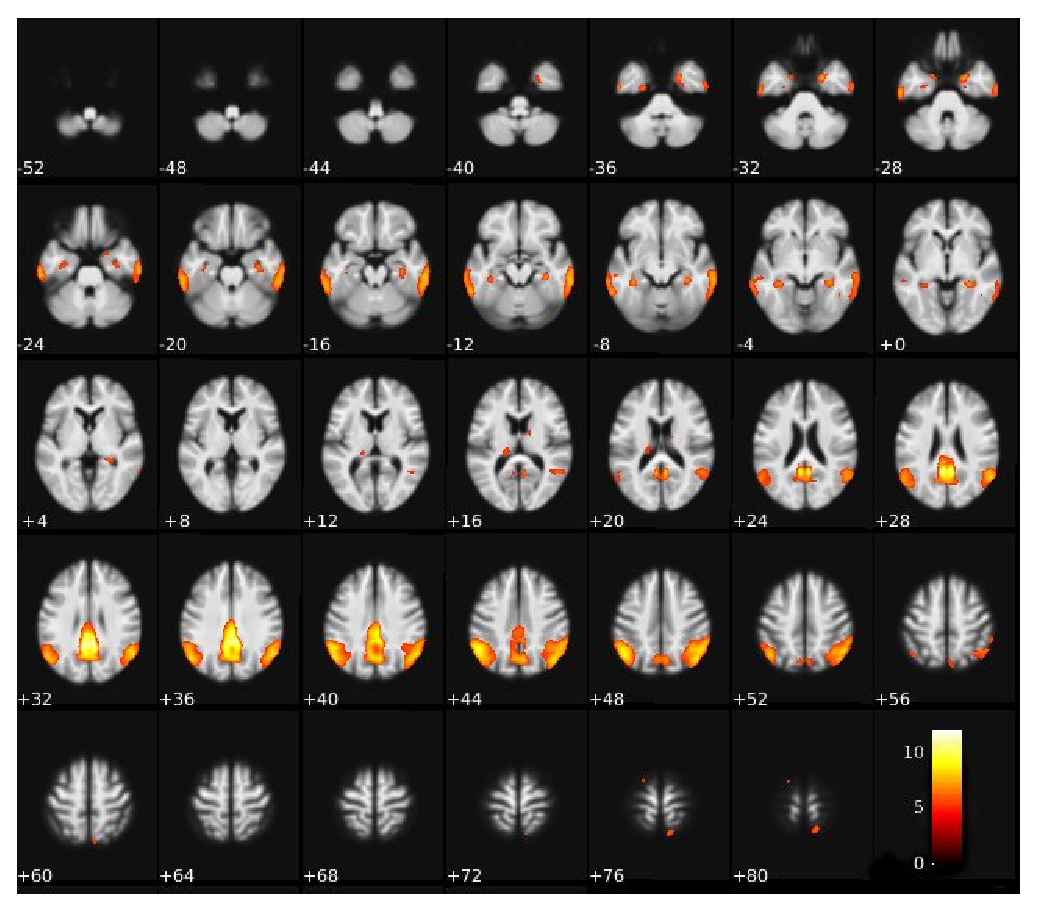
\includegraphics[width=\linewidth]{Graphics/ch2/example_SPM}
	\caption[Example of a \acs{SPM} analysis on a \acs{PET} dataset.]{Example of a \ac{SPM} analysis on a \ac{PET} dataset displaying the differences between \ac{AD} and \ac{CTL}, using $p<0.05$ and \ac{FWE} correction.}
	\label{fig:example_SPM}
\end{figure}

\ac{SPM} outputs maps like the one shown in Figure~\ref{fig:example_SPM}. There, significant $Z$-values according to a given threshold (\ac{FWE} uncorrected or corrected, see section~\ref{sec:multiplecomparisons}) are displayed over an anatomical reference.  The resulting maps allow a visual inspection of the significant brain areas, which can later be related to a certain disease or task. 

Although \ac{SPM}'s main feature is the estimation of differences, the term has been extended to cover the whole process performed by the \ac{SPM} software. That is, it generally involves registration to a template, intensity normalization, smoothing, the proper \ac{SPM} difference estimation and the display of the results. An overview of these procedures is provided at chapter~\ref{ch:preprocessing}. 

\subsection{\acf{VBM}}
\acf{VBM} can be considered an extention of \ac{SPM} applied to structural \ac{MRI} images \cite{Ashburner2000}. The procedure involves preprocessing (see chapter~\ref{ch:preprocessing}), where smoothing is applied to account for smaller anatomical differences. Afterwards, a \ac{GLM} is applied to each voxel in the images, and a $Z$-score map similar to Figure~\ref{fig:example_SPM} is produced. 

Smoothing is more important in \ac{VBM} than in regular \ac{SPM}, since \ac{MRI} images have higher resolution and are less noisy than functional images. Larger smoothing kernels will miss out smaller regions, while smaller kernel can lead to artifacts in the generated $Z$-maps, including misalignment of brain structures, differences in folding patterns or misclassification of tissue types \cite{Martinez-Murcia2016book}. Therefore, the kernel size must be carefully chosen, usually using a-priori knowledge about the regions affected, and always double checking for artifacts and reproducibility. 

The idea behind \ac{VBM} has been extended in a number of papers, using multivariate approaches that takes into account all voxels at once, and not their individual differences. Some of them include \ac{ICA} decomposition of the dataset and a posterior conversion to $Z$-scores in what was called Source Based Morphometry \cite{Xu2009}, or multidimensional Tensor Based Morphometry \cite{bossa2010tensor}. 

\subsection{The Multiple Comparisons Problem}\label{sec:multiplecomparisons}
The Multiple Comparisons problem arises when using hypothesis testing to assess statistical significance. This is widely used in neuroimaging, where statistical tests such as the $t$-Test or \ac{ANOVA} are used to quantify voxel-wise differences, and state their statistical significance, or $p$-value. The $p$-value, as described above, is the probability of any value being more extreme than a certain threshold under a given hypothesis. In our problem, given the $t$-value $T_i$ for the $i^{th}$ voxel ($i=1,\dots N$) of the images, and a threshold $T_{th}$ under the hypothesis $H$, the significance can be assessed by checking:
\begin{equation}\label{eq:pvalue}
P \left(T_i > T_{th}| H_0\right)<\alpha
\end{equation}
where $\alpha$ is the significance level. 

Choosing $\alpha$ is not trivial in neuroimaging. The use of the significance level $\alpha=0.05$ implies that any voxel with a $p$-value smaller than 0.05 is considered sufficient to reject the null hypothesis. This does not directly imply the necessity of accepting the alternative hypothesis $H_1$, although it is often thought so. Neither it yields the probability of the null hypothesis \cite{Dixon2003}. 

If we apply $p<0.05$ directly to a medical image of, for example, 300,000 voxels, that could mean the possibility of almost 15,000 voxels being false positives. Controlling the apparition of false positives when applying a massive univariate test is not trivial. It implies a balance between the true positive rate (sensitivity) or true negative rate (specificity), given that, for example, controlling the amount of false negatives will result in many false positives and vice-versa. 

Usually, two options for controlling the amount of false positives are given: the \acf{FWE} and the \acf{FDR}. The \ac{FWE} is the probability of obtaining at least one type I error. Mathematically, the null hypothesis for the $i^{th}$ voxel $H_{0i}$ states that there is no activation in that voxel. Therefore, the family-wise null hypothesis for our problem is:
\begin{equation}
H_0 = \bigcap_i H_{0i}
\end{equation}

If we reject a single null hypothesis ($T_i > T_{th}$), we reject $H_0$. Therefore, we want to control the probability of a single voxel being significant if the family-wise null hypothesis is valid:
\begin{equation}
P \left(\bigcup_i\{T_i > T_{th}\} | H_0\right)< \alpha
\end{equation}

In this case, we must obtain the critical value $T_{th}$, which is the higher $t$ value that matches that expression. Many options have been proposed to this problem, among them the conservative Bonferroni correction, methods that use random field theory or permutation tests. 

\subsubsection{The Bonferroni Correction}
The Bonferroni correction \cite{Shaffer1995} rewrites eq.~\ref{eq:pvalue} setting $\alpha=\frac{\alpha}{N}$ so that: 

\begin{equation}
P \left(T_i > T_{th}| H_0\right)< \frac{\alpha}{N}
\end{equation}

That way, using the Boole's inequality:
\begin{equation}
FWE \leq \sum_{i}^{N} \frac{\alpha}{N} = \alpha
\end{equation}

Therefore, we can comply with the imposed restriction for a maximum \ac{FWE}, or in our case, a maximum rate $\alpha$ of false positives. This is considered a rather conservative approach. In the example cited above, if we want to keep the \ac{FWE} below $0.05$, we should divide it by $N$, therefore obtaining a $T_{th}$ that makes $\alpha = 0.05/N = 1.67\times10^{-7}$. 

Other less conservative options try to compute a critical value $T_{th}$ that minimizes the \ac{FWE} using spatial information. This is the case of using an approximation of the distribution of the maximum statistic over the image, or the spatial correlation, including elements from random field theory (the approach used in \ac{SPM} \cite{spm_book}). 

\subsubsection{Random Field Theory}
In the random field approach, the maps of the statistic are treated, under the null hypothesis, as a lattice representation of smooth isotropic three dimensional random fields of test statistics. This approximation to the problem allow us to approximate the upper tail of the maximum distribution, the part needed for defining an event that occurs when the map exceeds the critical value $T_{th}$. Further information about random field theory and how it is applied to the \ac{SPM} software can be found at \cite{spm_book}. 

\subsubsection{FDR Controlling Procedures}
The other approach, based on the \ac{FDR}, aims at controlling the proportion of false positives in the total number of voxels declared significant. The most extended procedure for controlling the \ac{FDR} is that proposed by Benjamini and Hochberg \cite{Benjamini1995}. The Benjamini and Hochberg method start with calculating the $p$-values of all voxels and ranking them so that:
\begin{equation}
p_1 \leq p_2 \leq \dots \leq p_i \leq \dots \leq p_N \quad \forall i=1\dots N
\end{equation}

Let $q$ be the a maximum \ac{FDR} value that we can afford, for example $0.05$. For each $i$, we compute:
\begin{equation}\label{eq:bhFDRineq}
p_i \leq \frac{i}{N}q
\end{equation}

The maximum $i$ value that holds Eq.~\ref{eq:bhFDRineq} is used as $\alpha$, the significance level, and its corresponding statistical value ($T_i$ in the case of a $t$-test) is used as the critical value. This test, under the family-wise null hypothesis $H_0$, is equivalent to controlling the \ac{FWE}. However, \ac{FDR} methods are less conservative than other approaches such as the Bonferroni or other \ac{FWE}-based corrections, leading to a gain in statistical power. 


\subsubsection{Permutation Tests}
An empirical way to obtain $p$-values without relying on any parametric assumption is permutation testing \cite{Anderson2001,Winkler2014}. Permutation tests evaluate a statistic such as the F-statistic or the $t$-test using randomly target variables, in our case, the classes. The procedure is applied many times (up to 10,000), and for each permutation, only the maximum value of the computed statistic is considered. These values are used to build the null distribution, from which the family-wise corrected $p$-values are computed. Results obtained in permutation tests are comparable to those obtained using Random Field Theory \cite{Winkler2014}, and far less conservative than when applying the Bonferroni correction. 

\section{Machine Learning in Neuroimaging}\label{sec:machinelearning}
Machine learning is a current trend in neuroimaging. It provides computers with the ability to learn from data, using a set of statistical and computational tools. Rather than being explicitly programmed for a certain task, machine learning systems are able to find relevant data, discover patterns and predict the outcome of the input data. Its application to medicine is often known as \acf{CAD} \cite{Martinez-Murcia2016}. 

There are two major branches of machine learning: supervised and unsupervised learning. The former explores the patterns that lead to a certain outcome, whereas on the other hand, unsupervised learning explores the underlying structure of the data. Most of the \ac{CAD} systems rely on supervised learning, since their intention is to discover patterns that can effectively predict a disease. 

\begin{figure}[htp]
	\centering
	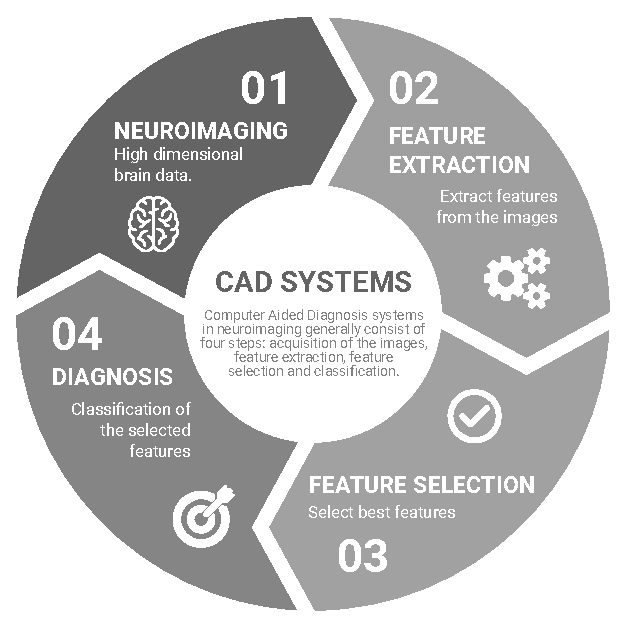
\includegraphics[width=0.5\linewidth]{Graphics/ch2/NI-CAD}
	\caption[Illustration of a typical neuroimaging \acs{CAD} system.]{Illustration of a typical neuroimaging \ac{CAD} system.}
	\label{fig:ni-cad}
\end{figure}

For simplicity, in this thesis, when talking about \ac{CAD}, we will always refer to automatic \ac{CAD} systems. That is, those that, once trained with previously known data, can predict the outcome of new, unseen data. A typical \ac{CAD} system, like the one in Figure~\ref{fig:ni-cad}, consists of input data (in our case, neuroimaging), feature extraction, feature selection and a classification step. The most basic is the \acf{VAF} approach, in which all voxels are considered as features, and then used as input to the classifier \cite{Stoeckel04}. However, many more advances can be made in this field by adding different combinations of feature selection and feature extraction algorithms. 

\subsection{\acf{VAF}}
\acf{VAF} \cite{Stoeckel04} is an example of the simplest \ac{CAD} system. It was originally proposed for evaluating and performing automatic diagnosis of \ac{AD} using functional \ac{SPECT} imaging. It uses a standard preprocessing (registration, intensity normalization) and a \ac{SVC} (See Appendix~\ref{ch:svm}) to predict the class of an image using all its intensities as features. Feature extraction, here, considers all voxels, and then there is no feature selection applied. 

It has been used in many works as a baseline \cite{Spetsieris2009,Salas-Gonzalez2009,Martinez-Murcia2016}, since it is comparable to the performance achieved by expert physicians using visual analysis \cite{Stoeckel04}. The weight vector of the \ac{SVC} can be inverse transformed to the dimension of the original images, and therefore provide a visual map that reflects the most influential voxels, in a similar way to the $Z$-maps of \ac{SPM} and \ac{VBM}. 

\subsection{Multivariate Analyses}\label{sec:mvanalyses}
Many improvements can be made to \ac{VAF} by adding and refining feature extraction and feature selection techniques. With this addition, we can avoid the Small Sample Size, in addition to the ability to discover higher level abstractions that can be more representative of the progression of the studied diseases. 

Feature extraction algorithms often change the strategy from a massive univariate approach, where a single feature is considered at each time, to multivariate analyses, where each feature can contain information from many voxels at the same time. Measures of total uptake of a given drug in nuclear imaging are a good example of this \cite{Zhou2007,Lozano2007}, but also the widespread Cortical Thickness \cite{Dale1999} provided by \textit{FreeSurfer} or the CAT12 toolbox of \ac{SPM}-12 (see Figure~\ref{fig:corticalthickness}). Cortical thickness is an estimation of the amount of \ac{GM} in a direction perpendicular to its surface. It first estimates the \ac{GM}-\ac{WM} and the \ac{WM}-\ac{CSF} separation surfaces, and then characterizes the thickness of the tissue, allowing a characterization of \ac{GM} differences such as atrophy or hypetrophy. 

\begin{figure}
\centering
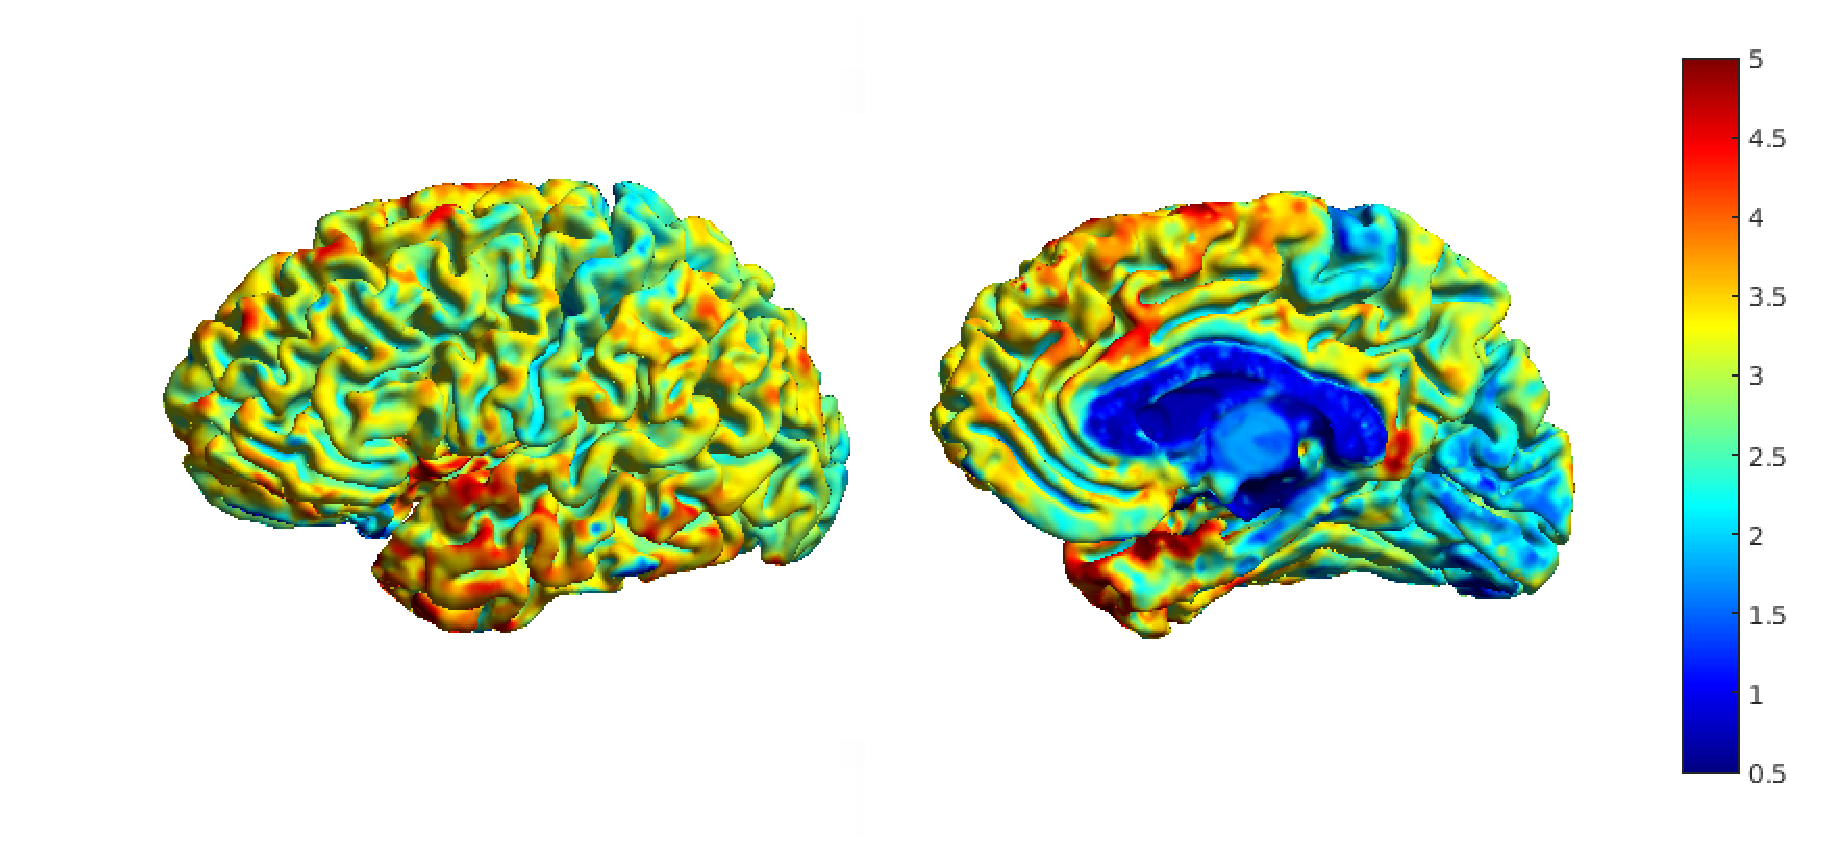
\includegraphics[width=0.8\linewidth]{Graphics/ch2/corticalThickness}
\caption[Example of the cortical thickness of a subject.]{Example of the cortical thickness of a subject, obtained with the toolbox CAT12 in SPM12.}
\label{fig:corticalthickness}
\end{figure}

Other more advanced algorithms are image decomposition techniques such as \ac{PCA} or \ac{PLS}, which have been extensively used in neuroimaging \ac{CAD} systems \cite{Spetsieris2009,Illan2011,Towey2011,Segovia2013,Khedher2015}. In these approaches, a given image can be represented as the linear combination of different components, and while the component loadings are common to all subjects, the weights of these components are unique to each patient. This allows us to identify the patterns that better discriminate between classes, leading to a more accurate diagnosis. 

For its part, feature selection refers to different strategies aimed at finding an optimal subset of the extracted features, according to a certain criterion. Irrelevant features are therefore discarded, making our models faster and more cost-effective \cite{Guyon03}. Feature selection algorithms are often subdivided in three approaches \cite{Martinez-Murcia2016b}: filters, wrappers and embedded approaches. 

Filters compute a feature relevance score from the data, which is then used to sort the different features. It is computed before the classification, and does not interact with it. Many scores can be derived from statistical features such as $\chi^2$, $t$-Test, Fisher's Discriminant Ratio (FDR) or others \cite{Martinez-Murcia2013255,Martinez-Murcia2016b}. The output of these tests is already a very extended tool in voxelwise analyses, as we commented in section~\ref{sec:vwanalyses}. 

Wrappers are similar to filtering methods, since they assign a certain score to each feature. But in contrast to filters, the score is computed by estimating the performance in a predictive model, such as classifiers \cite{Kohavi1995}. The most obvious measure here is accuracy, although other techniques such as Forward selection, backward elimination \cite{Guyon03}, genetic algorithms  \cite{Kohavi1995}, or the expectation-maximization algorithm \cite{Gorriz2009} have been used in the literature. And finally, embedded approaches use the very model that is being built to construct their optimal feature subset. 
